\documentclass[12pt]{article}
\usepackage[margin=1in]{geometry}
\usepackage{amsmath, amssymb, amsthm, graphicx, hyperref}
\usepackage{enumerate}
\usepackage{fancyhdr}
\usepackage{multirow, multicol}
\usepackage{tikz}
\pagestyle{fancy}
\fancyhead[RO]{Sicong Liu}
\fancyhead[LO]{MA-UY 2314: Discrete Mathematics}
\usepackage{comment}
\newif\ifshow
\showfalse
\begin{document}

\begin{center}
\textbf{\Large Homework 6}\\
\end{center}
\hrule
\vspace{0.2cm}
\begin{enumerate}

\item
\noindent 15.3 
\textbf{\begin{enumerate}[(a).]
\item equivalent relation
\item not equivalent relation $(3,3) \notin R$
\item not equivalent relation $(1,3) \in R, (3,1) \notin R$
\item not equivalent relation $(1,3) \in R, (3,1) \notin R$
\item equivalent relation
\item not equivalent relation $(4,4) \notin R$
\item equivalent relation
\end{enumerate}}

\item
\noindent 15.7
\textbf{\begin{enumerate}[(a).]
\item $\{1,2\}$
\item $\{4\}$
\item $\{120,121,122,123,124,125,126,127,128,129\}$
\item $\{you,brothers,sisters\}$
\item $\{all people with same birthday as me\}$
\item $\{\{1,2\},\{1,3\},\{1,4\},\{1,5\},\{2,3\},\{2,4\},\{2,5\},\{3,4\},\{3,5\},\{4,5\}\}$
\end{enumerate}}


\item
\noindent 15.8
\textbf{\begin{enumerate}[(a).]
\item 10
\item 366
\item 8
\item 50
\end{enumerate}}


\item
\noindent 15.9\\
NTS (1)$x \in [1] \longrightarrow x \in [3]$\\
NTS (2)$x \in [3] \longrightarrow x \in [1]$\\
Prove of (1): $x \in [1] \longrightarrow x=2k+1$ where $k \in \mathbf{z} \longrightarrow x=2(k-1)+3 \longrightarrow x \in [3]$\\
Prove of (2): $x \in [3] \longrightarrow x=2k+3$ where $k \in \mathbf{z} \longrightarrow x=2(k+1)+1 \longrightarrow x \in [1]$\\

\item
\noindent 15.15
\[
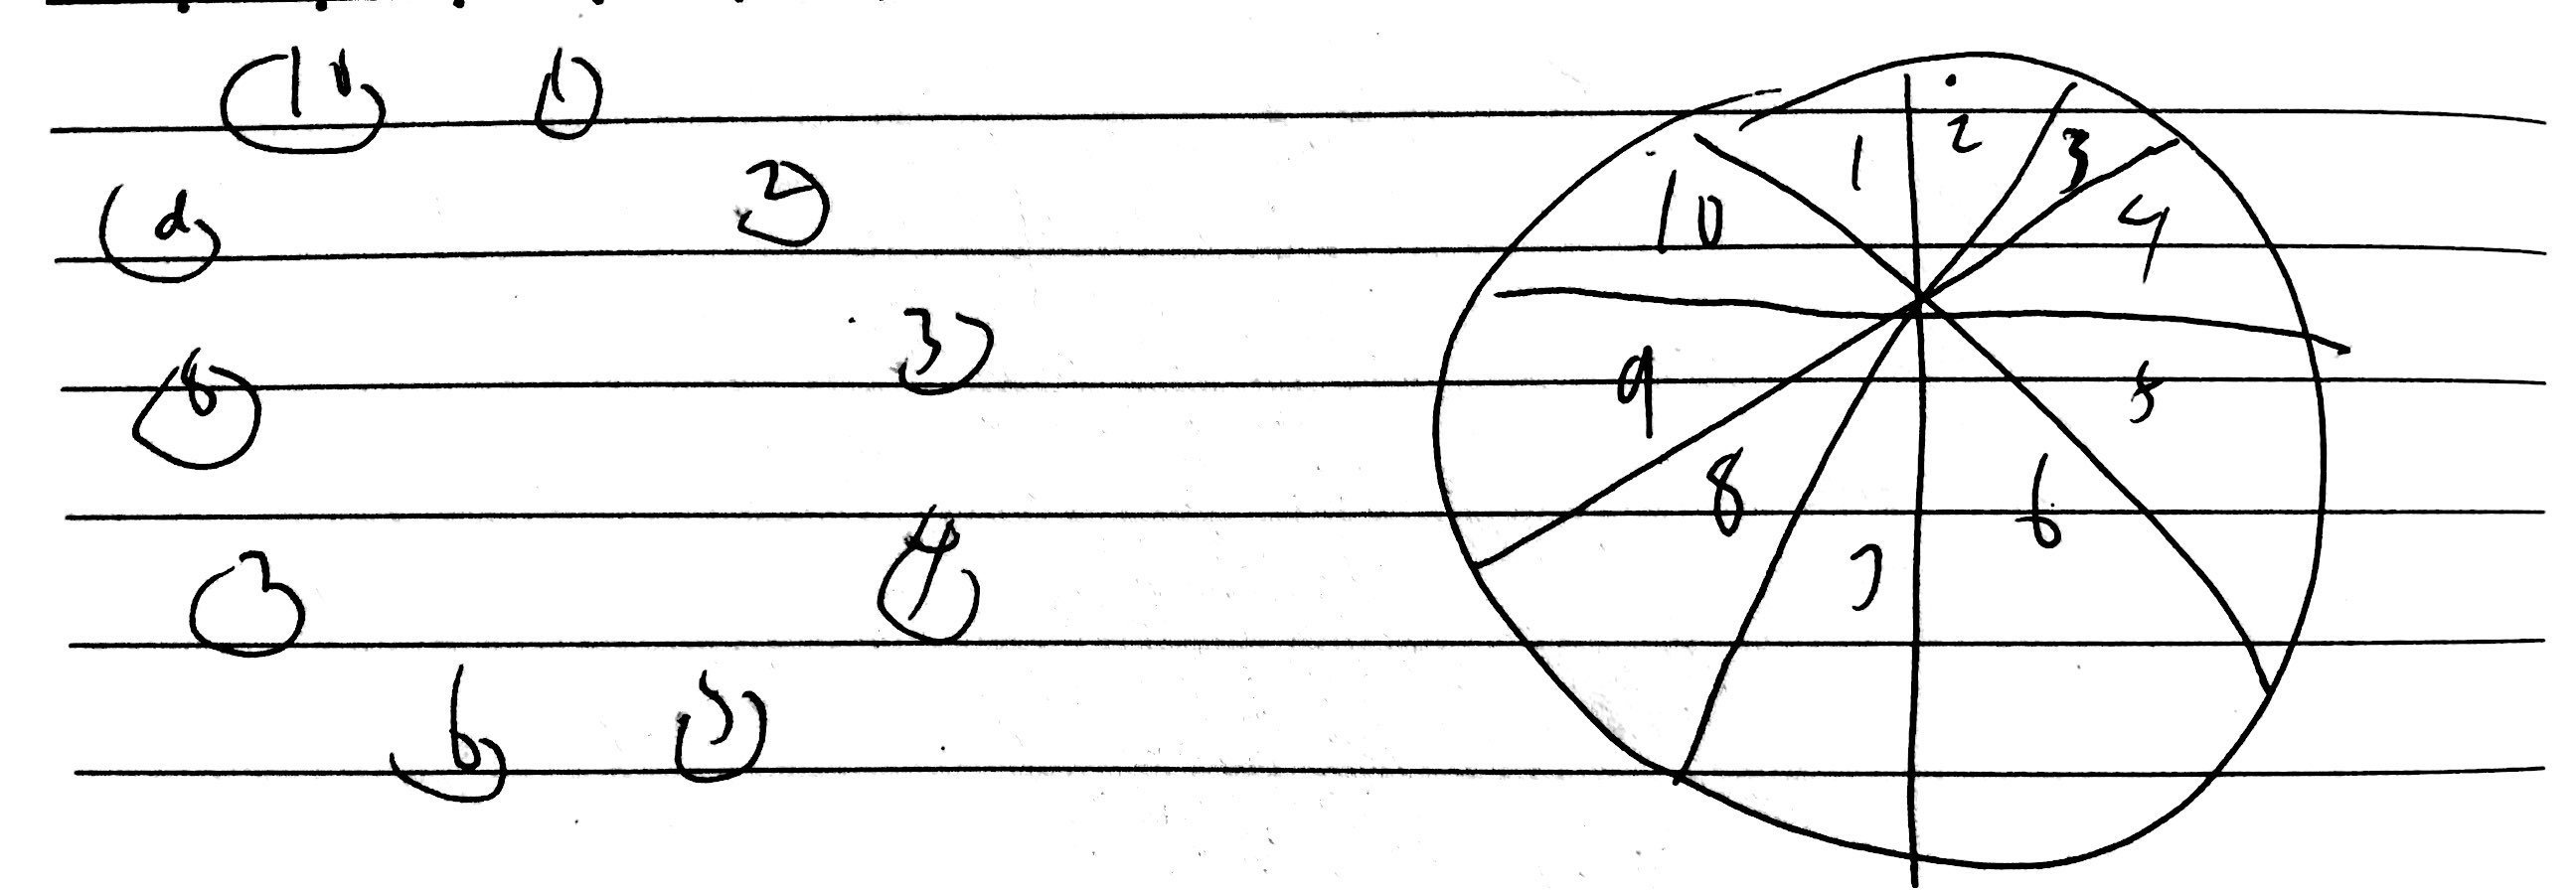
\includegraphics[width = 5in]{image.jpg} %your jpg file goes between the curly brackets.  To size it, play around with the syntax between the square brackets.  
\]

\item
\vspace{0.15in}
\noindent 16.1(a) $\{\{1\},\{2\},\{3\}\},\{\{1\},\{2,3\}\},\{\{2\},\{1,3\}\},\{\{3\},\{1,2\},\{1,2,3\}\}$\\

\noindent 16.1(b) $\{\{1\},\{2\},\{3\},\{4\}\}.\{\{1\},\{2,3,4\}\},\{\{2\},\{1,3,4\}\},\\
\{\{3\},\{1,2,4\}\},\{\{4\},\{1,2,3\}\},\{\{1,2\},\{3,4\}\},\{\{1,3\},\{2,4\}\},\{\{1,4\},\{2,3\}\},\{1,2,3,4\}$\\

\noindent 16.3 $5!/2!=60$

\item
\vspace{0.15in}
\noindent 16.8 $6! \times 5!$ 5! is the ways that men can form a circle, 6! is the ways that women can be arranged between men\\
\vspace{0.15in}
\noindent 16.9 $19!$\\
\noindent 16.12 $40!/((2!)^{20}20!)$ 20! ways to arrange the 20 groups, in 20 pairs, players can be arranged in $2^{20}$ ways\\ $40!3^{10}/((4!)^{10}10!)$ 10! ways to arrange the 10 groups, in 10 pairs, players can be arranged in $4^{10}$ ways, inside the group, 3 ways to arrange players\\
\item 
\noindent 16.14 $10!^{3}$ 10! for each position and 10! ways are repeated. $10!^{4}/10!$\\ 
\noindent 16.15 $2^{3}-1=7$,$2^{99}-1$\\
\noindent 16.16(a) $3^{100}$\\
\noindent 16.16(b) $3^{97}$ \\
\noindent 16.17 $100!/(20!(5!)^{20}) > 100!/(5!(20!)^{5})\\ \longrightarrow$ The number of partitions of A into 20 part of size 5 is greater.\\
\end{enumerate}
\end{document}